%%%%%%%%%%%%%%%%%%%%%%%%%%%%%%%%%%%%%%%%%%%%%%%%%%%%%%%%%%%%%%%%%%%%%%%%%%%
%% This file is part of the book
%%
%% Algorithmic Graph Theory
%% http://code.google.com/p/graph-theory-algorithms-book/
%%
%% Copyright (C) 2009, 2010 Minh Van Nguyen <nguyenminh2@gmail.com>
%%
%% See the file COPYING for copying conditions.
%%%%%%%%%%%%%%%%%%%%%%%%%%%%%%%%%%%%%%%%%%%%%%%%%%%%%%%%%%%%%%%%%%%%%%%%%%%

%% Chessboards where each square has dimensions 0.701125 x 0.701125.
%%
%% Solution for 4-queens.
\subfigure[$n = 4$]{
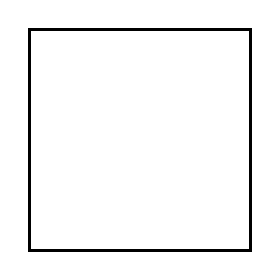
\begin{tikzpicture}
[borderdecorate/.style={-,very thick}]
%% chessboard with 4 queens
\node at (0,2.1) {\WhiteEmptySquare\WhiteQueenOnBlack\WhiteEmptySquare\BlackEmptySquare};
\node at (0,1.4) {\BlackEmptySquare\WhiteEmptySquare\BlackEmptySquare\WhiteQueenOnWhite};
\node at (0,0.7) {\WhiteQueenOnWhite\BlackEmptySquare\WhiteEmptySquare\BlackEmptySquare};
\node at (0,0.0) {\BlackEmptySquare\WhiteEmptySquare\WhiteQueenOnBlack\WhiteEmptySquare};
%% the boarders of the chessboard
\draw[borderdecorate]
(-1.405,-0.352) -- (-1.405,2.4525) -- (1.3995,2.4525) -- (1.3995,-0.352) -- cycle;
\end{tikzpicture}
}
\quad
%%
%% Solution for 8-queens.
\subfigure[$n = 8$]{
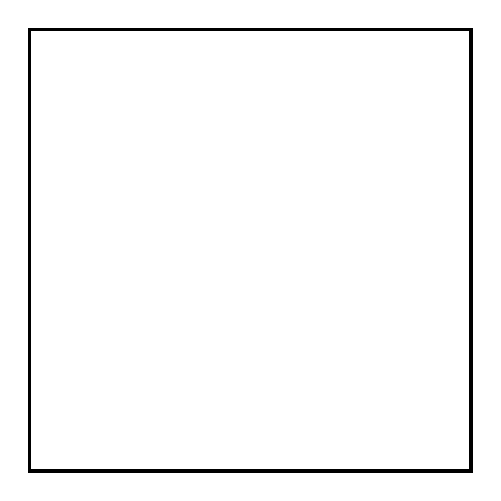
\begin{tikzpicture}
[borderdecorate/.style={-,very thick}]
%% chessboard with 8 queens
\node at (0,4.9) {\WhiteEmptySquare\BlackEmptySquare\WhiteQueenOnWhite\BlackEmptySquare\WhiteEmptySquare\BlackEmptySquare\WhiteEmptySquare\BlackEmptySquare};
\node at (0,4.2) {\BlackEmptySquare\WhiteEmptySquare\BlackEmptySquare\WhiteEmptySquare\BlackEmptySquare\WhiteEmptySquare\BlackEmptySquare\WhiteQueenOnWhite};
\node at (0,3.5) {\WhiteEmptySquare\BlackEmptySquare\WhiteEmptySquare\WhiteQueenOnBlack\WhiteEmptySquare\BlackEmptySquare\WhiteEmptySquare\BlackEmptySquare};
\node at (0,2.8) {\BlackEmptySquare\WhiteEmptySquare\BlackEmptySquare\WhiteEmptySquare\BlackEmptySquare\WhiteEmptySquare\WhiteQueenOnBlack\WhiteEmptySquare};
\node at (0,2.1) {\WhiteQueenOnWhite\BlackEmptySquare\WhiteEmptySquare\BlackEmptySquare\WhiteEmptySquare\BlackEmptySquare\WhiteEmptySquare\BlackEmptySquare};
\node at (0,1.4) {\BlackEmptySquare\WhiteEmptySquare\BlackEmptySquare\WhiteEmptySquare\BlackEmptySquare\WhiteQueenOnWhite\BlackEmptySquare\WhiteEmptySquare};
\node at (0,0.7) {\WhiteEmptySquare\WhiteQueenOnBlack\WhiteEmptySquare\BlackEmptySquare\WhiteEmptySquare\BlackEmptySquare\WhiteEmptySquare\BlackEmptySquare};
\node at (0,0.0) {\BlackEmptySquare\WhiteEmptySquare\BlackEmptySquare\WhiteEmptySquare\WhiteQueenOnBlack\WhiteEmptySquare\BlackEmptySquare\WhiteEmptySquare};
%% the boarders of the chessboard
\draw[borderdecorate]
(-2.8,-0.352) -- (-2.8,5.257) -- (2.809,5.257) -- (2.809,-0.352) -- cycle;
\end{tikzpicture}
}
